\subsection{Objetivos}

El desarrollo de una PCB se considera una de las partes esenciales de este proyecto y por lo tanto su importancia es máxima.

El objetivo principal que persigue el diseñar y construir una PCB en este proyecto es el de dotar al sistema de un centro de cómputo principal, el cual es utilizado para procesar las ordenes de S1, realizar los cálculos pertinentes y ejecutar las acciones necesarias sobre la estructura del brazo robótico.

Se considera  por lo tanto que la PCB es el centro de computo principal del sistema y por lo tanto se encarga de alojar el microcontrolador DSPIC, así como todos los periféricos necesarios para establecer la comunicación con S1, realizar el control de los actuadores y monitorizar el estado del manipulador.

En los siguientes apartados se detalla el proceso de diseño y construcción llevado a cabo para completar la PCB.

\subsection{Componentes principales}

El diseño de la PCB esta completamente estructurado según varios componentes principales, por lo tanto, en este apartado se describe cuales son, las decisiones que han llevado a incluirlos y sus funcionalidades principales dentro del proyecto.

En general se podría decir que los componentes de la PCB se clasifican en tres categorías principales:
\begin{itemize}
    \item Componentes de alimentación eléctrica.
    \item Microcontrolador y componentes auxiliares para su correcto funcionamiento.
    \item Periféricos destinados a control de actuadores y canales de comunicación.
\end{itemize}

En primer lugar, los componentes de alimentación eléctrica son aquellos que forman el circuito de alimentación del microcontrolador así como de los actuadores. El circuito eléctrico de alimentación de la PCB se ha diseñado para poder alimentar de forma simultánea al microcontrolador y a cada uno de los cuatro servomotores y por lo tanto, está formado por dos etapas:
\begin{itemize}
    \item La PCB recibe una tensión de entrada de 9V y una corriente de entre 1.8A - 2A mediante una clema. Posteriormente esta tensión de alimentación será reducida y adaptada para alimentar a cada una de las etapas de la PCB, es decir, al microcontrolador y servomotores.
    \item En la primera etapa se reduce el voltaje de alimentación principal a 6V y 0.4A aproximadamente para cada uno de los servomotores, utilizando para ello un regulador LM317 para cada servomotor. Esta alimentación se realiza mediante clemas, a las cuales se deben conectar la alimentación de los motores.
    \item En la segunda etapa se reduce el voltaje de alimentación principal a 3.3V y 0.15A aproximadamente con objetivo de alimentar el microcontrolador, utilizando para  ello un regulador LM317. Esta alimentación se realiza mediante pistas únicamente.
\end{itemize}

En segundo lugar, el microcontrolador y sus componentes auxiliares representan el núcleo de la PCB:
\begin{itemize}
    \item El DSPIC se encuentra localizado en el centro de la PCB y de el surgen todas las conexiones necesarias hacia los periféricos.
    \item Los componentes auxiliares del microcontrolador son componentes eléctricos que aseguran el correcto funcionamiento del DSPIC, así como su seguridad. En el caso específico de este microcontrolador, es necesario incluir varios condensadores en sus pines de alimentación.
\end{itemize}

En último lugar se detallan los principales periféricos que serán empleados:
\begin{itemize}
    \item Cristal de cuarzo: mediante este periférico se genera una señal de reloj precisa y de buena calidad, su frecuencia es de 7Mhz y sera recibida por el microcontrolador para ser usada como señal de reloj principal del sistema.
    \item Puerto de programación: mediante este periférico se puede conectar la sonda de programación del microcontrolador y por lo tanto es un elemento esencial.
    \item Puerto TRIS: mediante este periférico se pueden recibir señales digitales y analógicas las cuales son procesadas por el microcontrolador. En este proyecto se utiliza este periférico para monitorizar los finales de carrera de la estructura del brazo robótico.
    \item Puerto PWM: mediante este periférico se pueden generar señales PWM, las cuales son completamente necesarias para controlar los servomotores.
    \item UART: mediante este periférico se establece un canal de comunicación hardware con S1, el cual se usa para recibir ordenes, movimientos y realimentar su resultado de vuelta a S1.
    \item LEDS de estado: mediante este periférico se muestra el estado del sistema usando tres diodos LED.
\end{itemize}

Mediante esta descripción general de la PCB y sus componentes se pretende brindar una idea global de la misma, así como de cual es su papel dentro del proyecto. En los apartados siguientes se describe en términos técnicos los elementos de esta PCB, así como el proceso de diseño y fabricación llevado a cabo.

\subsection{Diseño lógico y diagrama esquemático}

El primer paso llevado a cabo durante el diseño de la PCB ha sido realizar un diseño lógico de alto nivel, en el cual se muestran las conexiones lógicas que existen entre los componentes; se trata por lo tanto del diseño con mayor nivel de abstracción y que tiene como objetivo establecer un diseño de primer nivel, es decir, la primera toma de contacto con el plano de la PCB.

El diseño lógico se lleva a cabo mediante un diagrama esquemático que contiene dos tipos de elementos: huella lógica de cada uno de los componentes y conexiones entre ellos. Este diagrama se ha llevado a cabo utilizando la herramienta Schematic Layout Editor incluida en KiCad.

El diagrama esquemático esta dividido en dos partes principales, las cuales facilitan la compresión del mismo:
\begin{itemize}
    \item Diagrama esquemático del circuito de alimentación.
    \item Diagrama esquemático del microcontrolador y sus periféricos.
\end{itemize}

En primer lugar se procede a describir detalladamente el diagrama esquemático del circuito de alimentación, el cual contiene las dos etapas de alimentación, incluyendo reguladores de voltaje LM317 y clemas.

La clema principal de alimentación recibe 9V y 1.8A aproximadamente. Esta alimentación debe ser provista externamente mediante una fuente de alimentación regulable o similares. 

Conectados directamente a la clema principal se encuentran los 5 reguladores de tensión que adaptan la tensión de alimentación a las dos etapas. Tal y como se puede observar, estos reguladores de tensión LM317 deben estar conectados de una forma particular para que cumplan su función correctamente, a continuación se detalla el proceso seguido para establecer su conexionado.

El funcionamiento del regulador LM317 es bastante común, se trata de un regulador de voltaje ajustable que recibe una tensión continua de entrada de entre 3V - 40V, y provee una tensión continua salida de entre 1.25V - 37V; la relación entre la tensión de entrada y salida depende de dos resistencias auxiliares. El conexionado sugerido por el fabricante es el siguiente y se ha obtenido del datasheet del regulador:

\begin{figure}[H]
    \centering 
    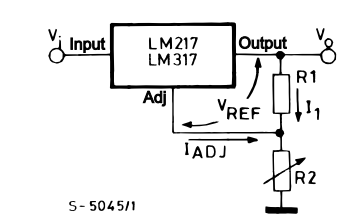
\includegraphics[width=.6\linewidth]{pictures/Lm317 conexionado.PNG}
    \caption{Diagrama de conexionado.}
    \label{fig:kdiagram}
\end{figure}


La ecuación de funcionamiento del regulador que ofrece el fabricante es la siguiente:
\begin{equation}
    V_{OUT} = V_{REF} \cdot ( 1 + \frac{R2}{R1}) + I_{ADJ} \cdot R2
\end{equation}

La ecuación anterior debe ser usada para realizar los cálculos pertinentes sobre el valor de las resistencias R2 y R1. Se pueden realizara además dos observaciones necesarias para la correcta aplicación de la ecuación anterior:
\begin{itemize}
    \item Se tiene que por definición, el fabricante establece el valor $V_{REF}$ en 1.25V
    \item Por motivos de construcción del regulador, la corriente $I_{ADJ}$ tiene un valor máximo de $100 \mu A$ y por lo tanto el término de la ecuación que la involucra puede ser despreciado.
    \item El valor recomendado por el fabricante para la resistencia R1 es de $240 \Omega$.
\end{itemize}

Se tiene por lo tanto que la ecuación funcional a utilizar en el cálculo de R1 y R2 es:

\begin{equation}
    V_{OUT} = 1.25 \cdot ( 1 + \frac{R2}{240}) 
\end{equation}

Teniendo en cuenta los voltajes de alimentación requeridos para las dos etapas de alimentación de la PCB, se han realizado los siguientes cálculos para los valores de la resistencia R2:
\begin{itemize}
    \item Etapa 1, alimentación de servomotores, 6V y 0.4A requeridos:
    \begin{equation}
        6 = 1.25 \cdot ( 1 + \frac{R2}{240}) 
    \end{equation}
    Se obtiene que el valor aproximado de R2 es $912 \Omega$, sin embargo por disponibilidad de materiales se escoge un valor de $R2 = 910 \Omega$, garantizando de esta forma un voltaje de salida de aproximadamente 5.989V.
    
    \item Etapa 2, alimentación del microcontrolador, 3.3 y 0.15A requeridos:
    \begin{equation}
        3.3 = 1.25 \cdot ( 1 + \frac{R2}{240}) 
    \end{equation}
    Se obtiene que el valor aproximado de R2 es $393.59 \Omega$, sin embargo por disponibilidad de materiales se escoge un valor de $R2 = 400 \Omega$, garantizando de esta forma un voltaje de salida de aproximadamente 3.34V.
\end{itemize}

Aplicando el conexionado recomendado por el fabricante y los cálculos para el valor de las resistencias se obtiene finalmente el diagrama esquemático del circuito de alimentación:

\begin{figure}[H]
    \centering 
    \includegraphics[width=.85\linewidth]{pictures/EsquematicoAlimentación.PNG}
    \caption{Diagrama esquemático del circuito de alimentación}
    \label{fig:kdiagram}
\end{figure}

%% foto de la parte izquierda

Es importante destacar tres aspectos:
\begin{itemize}
    \item La primera etapa de alimentación incluye clemas para su conexionado con los servomotores.
    \item La segunda etapa de alimentación incluye un puerto de cuatro pines, los cuales se usan para alimentar los micro-interruptores y el microcontrolador.
    \item El conexionado de todos los reguladores se ha realizado en paralelo, dedicando un regulador para cada servomotor, así como para el microcontrolador. El objetivo de esta configuración es garantizar una vía de alimentación independiente para cada componente, reduciendo las interferencias de alimentación entre los reguladores y, diferenciando la etapa de alimentación de los servomotores y microcontrolador.
\end{itemize}

En segundo lugar se procede a describir detalladamente el diagrama esquemático del microcontrolador y sus periféricos. A continuación se muestra el diagrama esquemático final y posteriormente se detallará cada uno de los periféricos:

\begin{figure}[H]
    \centering 
    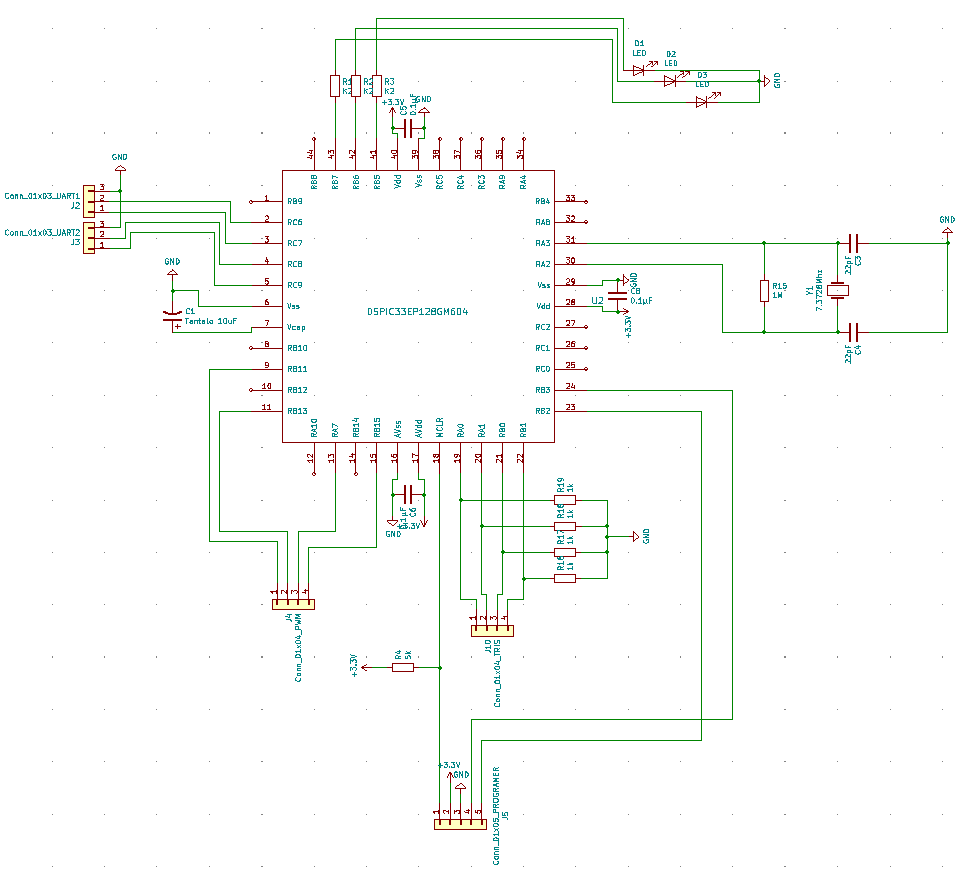
\includegraphics[width=.95\linewidth]{pictures/EsquematicoMicrocontrolador.PNG}
    \caption{Diagrama esquemático del microcontrolador y sus periféricos}
    \label{fig:kdiagram}
\end{figure}

Primeramente es importante describir los condensadores auxiliares necesarios para el correcto funcionamiento del microcontrolador, los cuales se encuentran conectados en los pines de alimentación del mismo. Su conexionado es sugerido por el fabricante en el datasheet según el siguiente esquema, se trata de la configuración mínima recomendada:

\begin{figure}[H]
    \centering 
    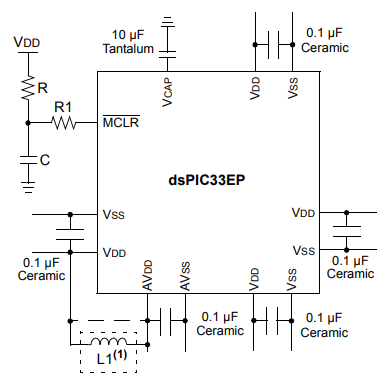
\includegraphics[width=.7\linewidth]{pictures/Minimun.PNG}
    \caption{Conexionado mínimo del microcontrolador}
    \label{fig:kdiagram}
\end{figure}

Todos los condensadores han sido conectados a los pines descritos por el fabricante y escogidos teniendo en cuenta las características técnicas de los mismos, también descritas en el datasheet.

A continuación se describe el conexionado del resto de puertos y periféricos:

\begin{itemize}
    \item Cristal de cuarzo: se trata del periférico que genera la señal de reloj principal del sistema, en este caso, su frecuencia es de 7.3728 Mhz y entra dentro del rango de válido mencionado en el datasheet.
    
    \begin{figure}[H]
    \centering 
    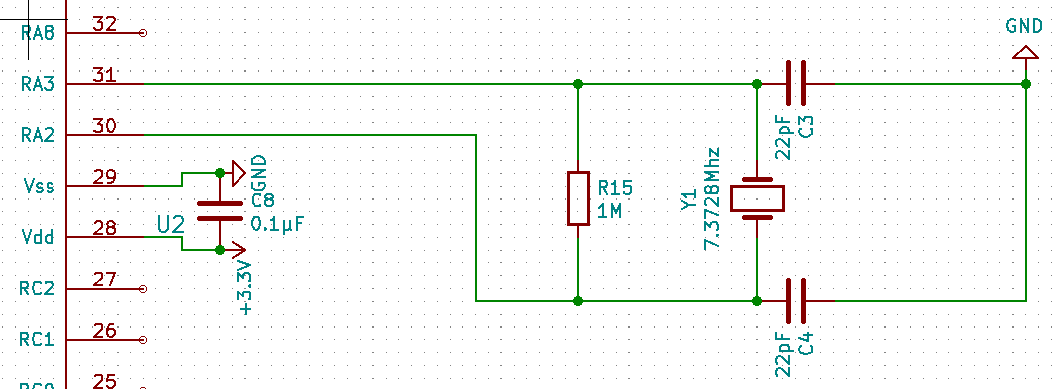
\includegraphics[width=.7\linewidth]{pictures/Cristal.PNG}
    \caption{Diagrama esquemático del conexionado del generador de señales}
    \label{fig:kdiagram}
    \end{figure}
    
    Su conexionado se realiza con los pines 32 y 31 del microcontrolador, siguiendo la estructura de la imagen anterior, empleando también una resistencia de $1 M \Omega$ y dos condensadores de 22 pF.
    
    \item Puerto de programación mediante sonda: se trata del puerto que permite conectar la sonda que introduce el código a ejecutar en el microcontrolador.
    
    El conector que recibe la sonda debe tener una estructura específica y se describe en el datasheet de la misma:
    
    \begin{figure}[H]
    \centering 
    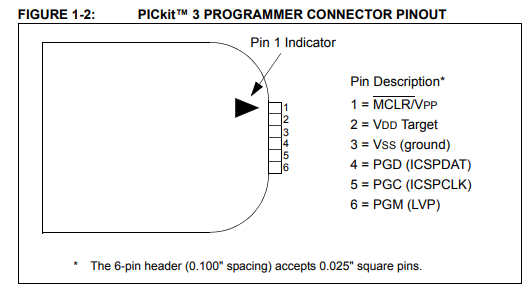
\includegraphics[width=.5\linewidth]{pictures/Sonda.PNG}
    \caption{Pinout del conector de la sonda de programación}
    \label{fig:kdiagram}
    \end{figure}
    
     Cabe destacar que el pin 18 o MCLR debe tener un conexionado específico en el que se emplea una resistencia pull-up; esta estructura de conexión se muestra en el datasheet del microcontrolador:
     
    \begin{figure}[H]
    \centering 
    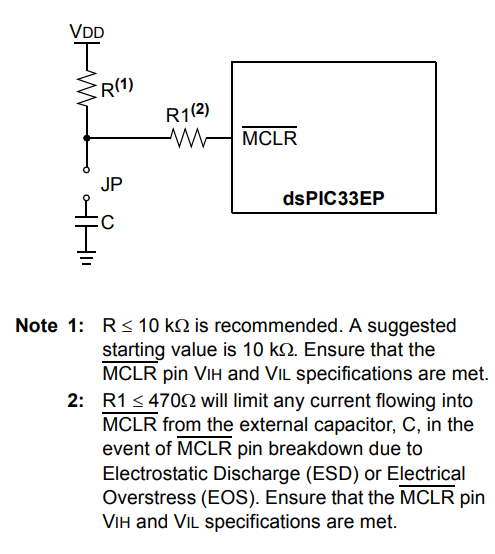
\includegraphics[width=.6\linewidth]{pictures/MCLR.PNG}
    \caption{Conexión del pin MCLR}
    \label{fig:kdiagram}
    \end{figure}
    
    En este proyecto se ha decidido no incluir el jumper sugerido para conexión del pin MCLR y por lo tanto R1 no se incluye en el diagrama esquemático.
    
    Teniendo en cuenta lo anteriormente mencionado, el conexionado final del puerto de programación mediante sonda es el siguiente:
    
    \begin{figure}[H]
    \centering 
    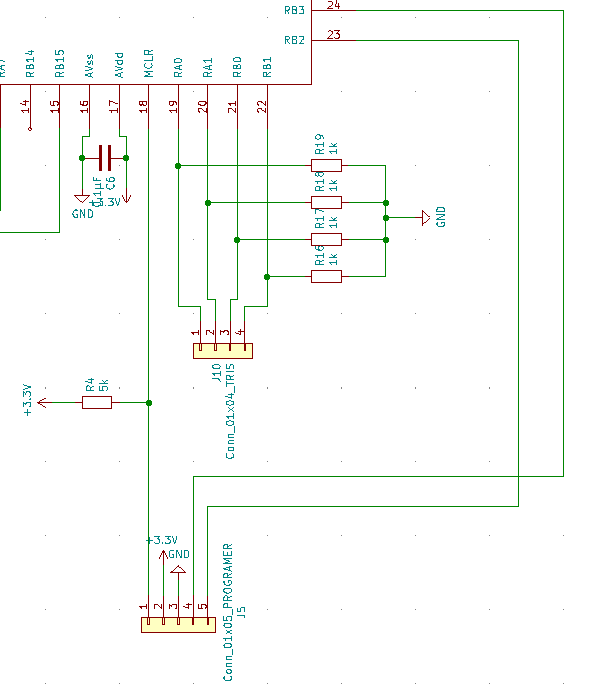
\includegraphics[width=.5\linewidth]{pictures/sonda.PNG}
    \caption{Diagrama esquemático del puerto de programación}
    \label{fig:kdiagram}
    \end{figure}
    
    \item Puerto TRIS: se trata del puerto al que se conectan los micro-interruptores que se utilizan en los finales de carrera de la estructura del brazo robótico.
    
    Para detectar si el brazo robótico se encuentra en uno de sus finales de carrera o zonas límite de movimiento, se utilizan unos micro-interruptores que al ser presionados por el manipulador, realizan cortocircuito. Mediante este cortocircuito y dado que estos micro-interruptores se encuentran conectados a los pines 19, 20, 21 y 22 del microntrolador, se puede realizar la lectura de dichos pines y detectar un nivel alto de 3.3V. De esta manera se consigue saber cuando el manipulador ha alcanzado o no un final de carrera.
    
    A continuación se muestra un esquema de lo mencionado anteriormente:
    
    %% meter foto de como funcionan los finales de carrera
    
    Mediante el conexionado anterior, si el micro-interruptor está abierto, se recibe un nivel bajo por el pin del microcontrolador; mientras que si el micro-interruptor está cerrado se recibe un nivel alto por el pin del microcontrolador. 
    
    Cabe destacar que tanto la resistencia pull-down como la conexión a tierra se incluyen en la PCB, sin embargo los micro-interruptores y su conexión a VDD se encuentran localizados en la estructura del brazo robótico. 
    
    El diagrama esquemático que implementa esta funcionalidad es el siguiente:
    
    \begin{figure}[H]
    \centering 
    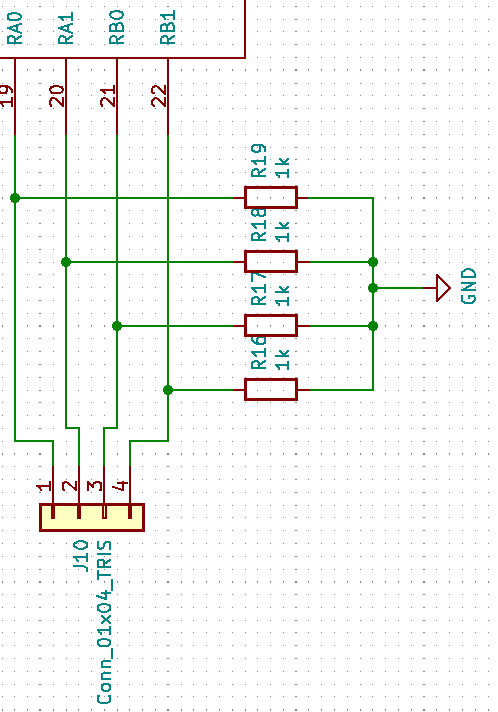
\includegraphics[width=.4\linewidth]{pictures/TRIS.PNG}
    \caption{Diagrama esquemático del puerto TRIS}
    \label{fig:kdiagram}
    \end{figure}
    
    
    
    \item Puerto PWM:
    
    \item UART:
    
    \item LEDs de estado:

    
    
\end{itemize}


    
\subsection{Diseño y Diagrama físico}

\subsection{Conexionado y enrutado mediante pistas}

\subsection{Verificaciones del diseño final}

\subsection{Decisiones críticas durante el desarrollo}

\subsection{Construcción}

